\documentclass{article}
\usepackage{amsmath, amssymb, amsthm, amsfonts}
\usepackage{fullpage}
\usepackage{graphicx}

\newtheorem{theorem}{Theorem}
\newtheorem{lemma}{Lemma}
\newtheorem{corollary}{Corollary}
\newtheorem{definition}{Definition}
\newtheorem{proposition}{Proposition}
\newtheorem{procedure}{Procedure}
\newtheorem{construction}{Construction}
\newtheorem{example}{Example}
\newtheorem{remark}{Remark}
\newtheorem{claim}{Claim}

\newcommand{\Rea}{{\mathbb R}}
\newcommand{\Int}{{\mathbb Z}}
\newcommand{\Rat}{{\mathbb Q}}
\newcommand{\Cmp}{{\mathbb C}}
\newcommand{\Nat}{{\mathbb N}}

\setlength{\oddsidemargin}{.25in}
\setlength{\evensidemargin}{.25in}
\setlength{\textwidth}{6.25in}
\setlength{\topmargin}{-0.0in}
\setlength{\textheight}{8.9in}

\renewenvironment{proof}{\noindent{\bf Proof:} \hspace*{1mm}}{
	\hspace*{\fill} $\Box$ }
\newenvironment{proof_of}[1]{\noindent {\bf Proof of #1:}
	\hspace*{1mm}}{\hspace*{\fill} $\Box$ }
\newenvironment{proof_claim}{\begin{quotation} \noindent}{
	\hspace*{\fill} $\diamond$ \end{quotation}}

\newcommand{\handout}[6]{
   \renewcommand{\thepage}{#1-\arabic{page}}
   \noindent
   \begin{center}
   \framebox{
      \vbox{
    \hbox to 5.78in { {\bf #2} \hfill #3 }
       \vspace{4mm}
       \hbox to 5.78in { {\Large \hfill #4  \hfill} }
       \vspace{2mm}
       \hbox to 5.78in { {\it #5 \hfill #6} }
      }
   }
   \end{center}
   \vspace*{4mm}
   \medskip {\large \noindent {\bf NOTE: } \bf The content of these notes has not been formally reviewed by the lecturer. It is recommended that they are read critically.}
}

\newcommand{\lecture}[3]{\handout{#1}{Ubinet, Distributed Optimization and Games 2016-2017}{#2}{Lecture #1}{Lecturer: Giovanni Neglia}{Scribe: #3}}




\newcommand{\x}{\mathbf{x}}
\newcommand{\y}{\mathbf{y}}
\newcommand{\z}{\mathbf{z}}
\newcommand{\blambda}{\boldsymbol{\lambda}}
\newcommand{\bmu}{\boldsymbol{\nu}}
\usepackage{color}

\begin{document}
%header --- replace with appropriate values
\lecture{2b}{December 14, 2016}{Arthur Finkelstein, Remy Garcia}

%start notes here
\section{Introduction}

In the previous lesson, we looked into the example of an electrical network and showed that a simple local policy for an agent, in our case an electron, can lead to the optimization of a large distributed problem which is the minimization of energy loss in the  network. In this lesson, we consider a road traffic model to demonstrate that choosing local policies is not trivial and how potential wrong choices can lead to poor system behaviour. Moreover we solve the more general problem which arises from our road network and present how local policies in such cases should be correctly chosen.

\section{Problem Definition}
We consider an oriented graph (e.g.\ the road-traffic graph of a city) like in Figure~\ref{fig:1}. From now on we look at this problem as a routing problem.
\begin{figure}[h!]
\centering
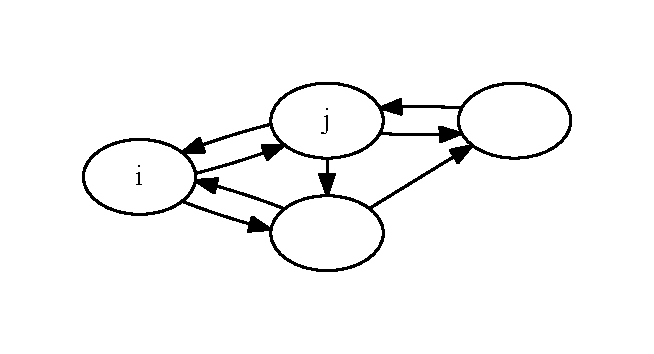
\includegraphics[scale=.7]{fig1.pdf}
\caption{Oriented graph of a city}
\label{fig:1}
\end{figure}

We have a set of directed links $E$ which are the connections between the nodes of the graph and a set of \textit{source-destination} pairs $S$, where we have $s \in S$ such that $s = (i,j$) represents the agents wanting to travel from node $i$ to $j$. Moreover we denote by $R$ the set of all routes.

For each $s \in S$ we define $R(s)$ to be the set of routes connecting the \textit{source-destination} pair and $f_s$ to be the amount of traffic to route on $s$. Also $s(r)$ is the \textit{source-destination} pair connected by $r \in R$. Since a given $f_s$ can be split over various routes, we denote by $x_r$ the amount of traffic of $s(r)$ that takes route $r$ i.e.\ $\sum\limits_{r \in R(s)}^{} x_r = f_s,\ \forall s$ with $x_r \ge 0$.

Finally, we define $y_l$ to be the amount of traffic on link $l \in E$ due to all routes passing by $l$, i.e.\ $y_l=\sum\limits_{r | l \in r} x_r$. On each link $l$ there exists a delay per unit of traffic which is a function of the traffic on that link that we denote by $D_l(y_l)$. The delay function is assumed to be convex, increasing and its second derivative to exist.\\

Thus the problem consists of minimizing the overall delay experienced by the agents.\\

The optimization problem can be modeled as follows:
\begin{equation}
\begin{aligned}
& {\text{minimize}}
    & &  \sum_{l \in E} y_{l} D_{l}(y_{l}) \\
& \text{subject to}
& & \sum_{r \in R(s)} x_{r} = f_{s},\ \forall s \in S\\
&       & &  y_{l} = \sum\limits_{r|l \in r} x_{r},\ \forall l \in E\\
&      &&  x_{r} \geq 0,\ \forall r \in R\\
\end{aligned}
\label{e:prob}
\end{equation}

This problem happens to be convex.

\begin{proof}
	We first observe that the constraints identify a convex set $\{x_r \ge 0 \}$.
	
        We know that $D_l$ is increasing and convex. This means that for all $y_l$ we have $D_l'(y_l) \ge 0$ and $D_l''(y_l) \ge 0$.

        We know that $y_lD_l(y_l)$ is convex iff its second derivative is nonnegative.

        We start by computing the first derivative. $(y_lD_l(y_l))' = D_l(y_l) + y_lD_l'(y_l)$ where $D_l(y_l) \ge 0$ and $y_lD_l'(y_l) \ge 0$. Thus $(y_lD_l(y_l))'$ is nonnegative.

        Then we compute the second derivative. $(y_lD_l(y_l))'' = D_l'(y_l) + y_lD_l''(y_l) + D_l'(y_l) = 2D_l'(y_l) + y_lD_l''(y_l)$ where $2D_l'(y_l) \ge 0$ and $y_lD_l''(y_l) \ge 0$. Thus $(y_lD_l(y_l))''$ is nonnegative.

        Hence $y_lD_l(y_l)$ is convex and it implies that $\sum\limits_{l} y_{l}D_{l}(y_{l})$ is also convex and thus this problem is convex.
\end{proof}

\section{Naive solution}

One naive solution for this problem would be that each agent tries to minimize its own delay, and from this we could hope that the total delay would be minimized. Therefore we are going to check if this solution is indeed the optimal one and, if it is not so, how far off we are from the optimal.

\subsection{A first example: parallel links with linear delay functions}

\begin{figure}[h]
\centering
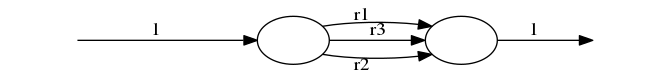
\includegraphics[scale=0.5]{output.png}
\caption{Our specific network}
\end{figure}

With this specific example each different edge has a specific delay equal to $ D_i = \alpha_i \times y_i$.

In this setting, if every agent minimizes its own delay, we can expect that at the equibrium all the routes have the same delay. Indeed, if it were not so, some of the agents will find more convenient to move from a route with higher delay to a route with lower delay.

We can now check if this equilibrium corresponds to the solution minimizing the total delay.
The total delay is $\sum\limits_{i=1}^{3} (\alpha_i \times y_i) \times y_i = \sum\limits_{i=1}^{3} \alpha_i \times y^2_i $, and we can see that this function is the same as the model we studied in the first lecture.

We can then compare our network to an electrical network with three different resistances in parallel, and from our previous lecture we know that at the optimum, the currents are such that $ \Delta V = I_1 R_1 = I_2 R_2 = I_3 R_3 $ with $I_i = y_i $ and  $ R_i = \alpha_i $, so at the optimal solution $y^*_i$ we have then $\alpha_1 \times y^*_1 = \alpha_2 \times y^*_2 = \alpha_3 \times y^*_3$ which is  $ D_1(y^*_1) = D_2(y^*_2) = D_3(y^*_3)$.

%This result can be easily understood with the fact that each car at the beginning will take the path with the least delay and once this delay becomes bigger than the delay of either of the other path we will take this path, and so on, this will create a situation of equilibrium in regard to the delays of each route.

The conclusion is then that, at least in this setting, if each agent selects the route with minimum delay, then the system converges to a configuration with minimum global delay.

\subsection{Pigou's example}

\begin{figure}[h]
\centering

\includegraphics[scale=0.5]{output2.png}
\caption{Our general network}
\end{figure}

We are now going to extend the previous example with delay functions that are not linear, we have then $D_1(y_1) = 1$ and $D_2(y_2) = y^n_2 $, because this function relates the most to how delay affects routing in a real world scenario. This example is known as the Pigou's  example.

The comparison between the two delay function gives us the following graphic.

\begin{figure}[h]
\centering
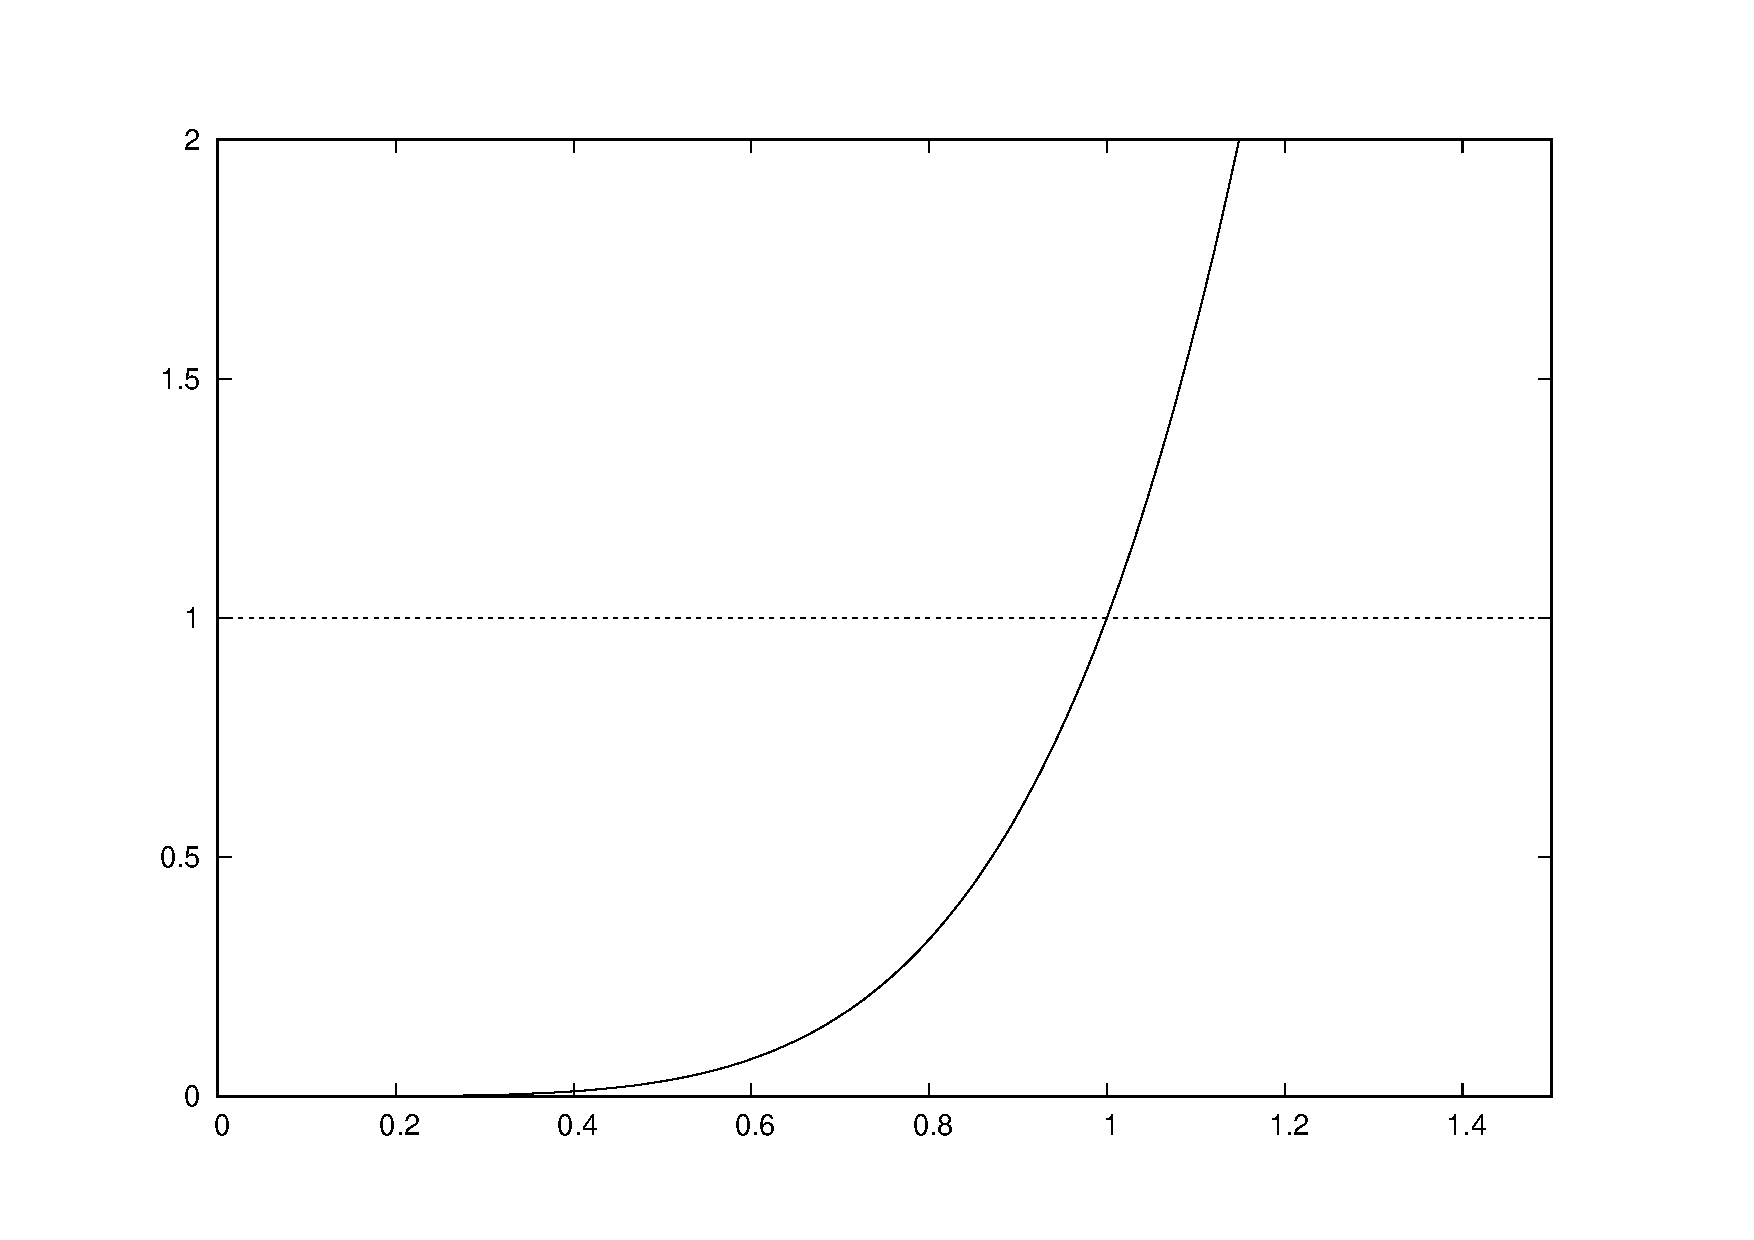
\includegraphics[scale=0.2]{exo2.pdf}
\caption{Our general network}
\end{figure}

We now put our naive solution in this example with each person minimizing his or her delay. We get $y^1_1 = 0$ and $y^1_2 = 1$ because the second link is always the most attractive with regard to the delay. The total delay is then $D_t(1) = 1 \times 0 + 1^n \times 1 = 1$.

We now solve the problem. Consider a general splitting of the traffic between the two links and denote by $\alpha$ the amount of traffic on link $2$. The traffic on link $1$ is then $1-\alpha$ and the total delay is  $D_t(\alpha ) = (1 - \alpha ) \times 1 \times \alpha \times \alpha ^n$. We know that to find the minimum we look for: $$D'_t(\alpha ) = 0 \iff -1 + (n + 1) \times \alpha ^n \iff \alpha ^* = \frac{1}{{\sqrt[n]{n+1}}}$$ Thus we know that the optimal quantity of traffic is $\alpha ^*$. Now we will check if the delay we got from the naive solution is optimal or not.

The optimal delay is: $$D_t(\alpha ^*) = 1 - \alpha ^* + \alpha ^{*^{n+1}} = 1 - \frac{1}{{\sqrt[n]{n+1}}} + \frac{1}{{\sqrt[n]{n+1}}} * \frac{1}{n+1} = 1 - \frac{1}{{\sqrt[n]{n+1}}} * \frac{n}{n+1}$$ Thus we can deduce that for every $ n > 0$ the delay is strictly less than 1. Therefore the naive local rule does not lead to minimize the total delay. Nevertheless,  if the corresponding total delay is close enough to the optimal one, it would still be acceptable.

For this we compute the price of anarchy: $$ \frac{D_t(\alpha ^1)}{D_t(\alpha ^*)} = \frac{1}{1 - \frac{1}{{\sqrt[n]{n+1}}} * \frac{n}{n+1}} \underset{n \to \infty}\rightarrow +\infty$$ Thus the naive solution gives us a delay that is arbitrarily bigger than the optimal one so our solution is unfortunately pretty poor.

After having ruled out the naive local rule to select the route with minimum delay, we move to study directly the original problem.

\section{Solving Problem~\eqref{e:prob} by the Lagrange multipliers method}
Observe that the feasible set is compact (closed and bounded). In fact the constraints define a bounded polyhedral set because each variable $x_r$ is bounded:
\begin{equation}
0 \leq x_r \leq \underset{s \in S}{\text{max}} {f_s} \;\; \forall r \in R
\end{equation}
Because the feasible set is compact and the objective function is continuous, then the problem admits a global minimum. 

Moreover, all the hypotheses of theorem $1$ from lesson 2a are satisfied and then we can find a point of global minimum using the Lagrange multiplier method.
%We can observe that the objective function of our optimization problem \eqref{e:prob} is convex. Indeed:
%\begin{equation}
%f(x) = y_l D(y_l) \Rightarrow f'(x) = y_l D'(y_l) + D(y_l) \Rightarrow f''(x) = y_l D''(y_l) + D'(y_l) + D'(y_l)
%\end{equation}
%We know that $D'(y_l)$ and $D''(y_l)$ are nonnegative, on the hypothesis that $D(y_l)$ is convex. Thus each term of $f''(x)$ is nonnegative and the sum of nonnegative terms is nonnegative, hence the objective function is convex.\\
%Another observation that we make is that each constraint is linear and that they define a set which is compact. Indeed, each variable $x_r$ is bounded:
%\begin{equation}
%0 \leq x_r \leq \underset{s \in S}{\text{max}} {f_s} \;\; \forall r \in R
%\end{equation}
%so the set defined is closed and bounded and then the problem admits .\\\\
%Considering the previous observations we can apply the \emph{lagrange multipliers method} while using  theorem $(1)$ from the lesson 2. 
In particular we consider as polyhedral set $X=\{x_r \ge 0, \forall r \in R\}$ and we define two set of multipliers:
\begin{enumerate}
        \item one for each source-destination pair, $\lambda_s$, $ \forall s \in S$ and
        \item one for each link, $\nu_l$, $\forall l \in E$.
\end{enumerate}
Let $\z^* = {\x^* \choose \y^*}$ denote a global minimizer, then, because of theorem~1,  there exist $\lambda_s^*$, $\forall s \in S$ and $\nu_l^*$, $\forall l \in E$ such that:
\begin{enumerate}
\item $\x^*$ and $\y^*$ are feasible,
\item $\nabla_\z L(\z^*,\blambda^*,\bmu^*)^T (\z - \z^*) \ge 0,  \;\; \forall \z \in \{{\x \choose \y} ,\; \x \ge 0  \}$.
\end{enumerate}
The Lagrangian function results:
\begin{equation} 
L(z,\lambda,\nu)= \sum_{l \in E}  y_l D(y_l) + \sum_{s \in S} \lambda_{s} \left(f_s - \sum_{r:s(r)=s} x_r\right) + \sum_{l \in E} \nu_l \left(\sum_{r:l \in r} x_r - y_l\right) 
\end{equation}
When we differentiate it, we obtain:
\begin{equation}
\label{e:derivatives}
\begin{aligned}
        \frac{\partial L}{\partial y_{\bar{l}}}=D(y_{\bar{l}})+  y_{\bar{l}} D'(y_{\bar{l}}) -  \nu_{\bar{l}}  &&&&& &&&&& \frac{\partial L}{\partial x_{\bar{r}}}=- \lambda_{s(\bar{r})} + \sum_{l \in \bar{r}} \nu_l
\end{aligned}
\end{equation}


Observe that we can both increase and decrease $y^*_{\bar l}$ without going out of the polyhedral set $X$, i.e both ${\x^* \choose \y^*}+ \Delta y_{\bar l}{\mathbf 0 \choose \mathbf e_{\bar l}} $ and ${\x^* \choose \y^*}- \Delta y_{\bar l}{\mathbf 0 \choose \mathbf e_{\bar l}} $ belong to $X$, where $\mathbf e_{\bar l}$ is the vector with the $\bar l$-th component equal to one and all the others equal to 0. Then, from the condition on the gradient of the Lagrangian, it follows:
$$ \frac{\partial L}{\partial y_{\bar l}}\bigg|_{\z^*} \Delta y_l \geq 0,$$
$$ \frac{\partial L}{\partial y_{\bar l}}\bigg|_{\z^*} \times (-\Delta y_l) \geq 0.$$
From these two results we can see that $\frac{\partial L}{\partial y_l}$ is equal to zero.


If $x^*_{\bar r}>0$ it is possible to both increase and decrease it. In such case we get as above:
$$ \frac{\partial L}{\partial x_{\bar r}}\bigg|_{\z^*}  = 0.$$
Instead if $x^*_r=0$, it is only possible to increase it and we
 get:
$$ \frac{\partial L}{\partial x_{\bar r}}\bigg|_{\z^*} \ge 0$$
%if there is traffic on that route $x_r = 0$ and if there is no traffic then $x_r \geq 0$.

From \eqref{e:derivatives}, these conditions can be rewritten as follows in terms of the Lagrange multipliers:
\begin{equation}
\label{e:lambda}
\lambda^*_s(r)
\begin{cases}
= \sum_{l \in r} \nu^*_l & \mbox{if } x_r > 0,\\
\leq \sum_{l \in r} \nu^*_l & \mbox{if } x_r = 0,
\end{cases}
\end{equation}
%and the quantity $\nu_l$ results:
\begin{equation}
\label{e:nu}
\nu^*_l = D(y_l)+  y_l D'(y_l).
\end{equation} 

We can interpret these equations as follows. First, each multiplier  $\nu_l^*$ can be interpreted as a cost associated to link $l$, that is a function of the total traffic on the link. We can then associate a cost to each route as the sum of the link costs. Equation~\eqref{e:lambda} then tells us that for each source-destination pair $s$ all the routes used have the same route cost equal to $\lambda_s^*$ and this is the minimum route cost (all the routes that are not used have higher route cost).

The optimal solution can then be achieved in a distributed way similarly to our initial naive solution. Costs for each link can be computed, aggregated over each route and propagated to each agent, who should then choose the route with minimum cost. The difference is in the right cost to consider: the link cost is composed of the delay (i.e. $D(y_l)$) plus the additional term $y_l D'(y_l)$. 

\begin{figure}[h!]
\centering
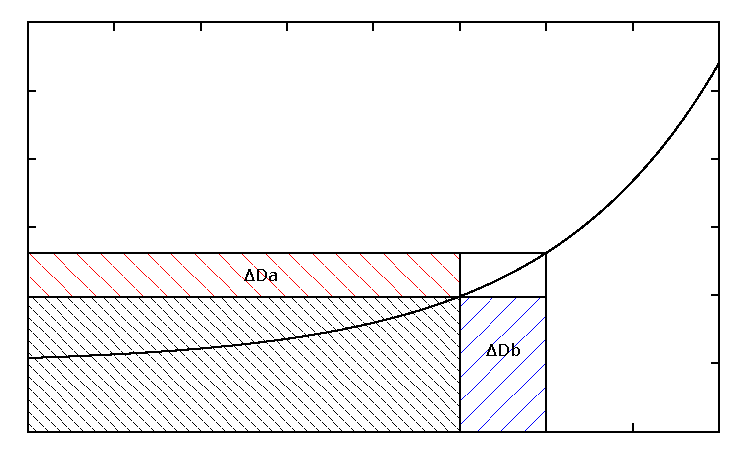
\includegraphics[scale=.7]{fig3.pdf}
\caption{Additional term representation}
\label{fig:3}
\end{figure}

In order to interpret the meaning of this additional term, let us consider what is the effect of adding some  traffic $\Delta y$ to a given link $l$.
In Figure~\ref{fig:3} the initial link delay experienced by all the users is denoted by the black area. When computing the new total delay, we need to consider the red area, $\Delta D_{a}$ and the blue area, $\Delta D_{b}$, where $\Delta D_{a} = y_l D'(y_l ) \Delta y$ and $\Delta D_b = \Delta y D(y_l)$. %Then we have $\Delta D = \Delta y (D(y_l')+y_l'D'(y_l'))$, the weight of the link. 
We observe that $\Delta D_{b}$ is the total delay experienced by this additional traffic and this is what the corresponding users would take into account in their choice to move to link $l$.
Instead, $\Delta D_{a}$ is the total delay increase for the traffic already on link $l$. Then, considering the additional term $y_l D'(y_l)$ in the link cost corresponds to each user taking into account the delay increase that his choice would cause to the other users.

While we can assume that each user is immediately sensitive to the delay he experiences, we can wonder how we can make him responsive also to the additional term $y_l D'(y_l)$. A possibility in a transportation scenario is to add some tolls, so that  drivers are encouraged to have a more desirable behaviour. We can revisit the example in the previous section and  add the toll $y_l D'(y_l)$ at the cost of each link. Each user experiences then two new costs for traveling the two paths. 
 $C_{upper}=1 + y_{upper} D'(y_{upper})= 1$ and   $C_{lower} = y_{lower} + y_{lower} D'(y_l)= 2y_{lower}$. Now the drivers choose the link where the total cost, delay plus toll, is minimum and the final solution is that half of the drivers choose the lower link and the others choose the upper link, that is the optimal solution for Problem \eqref{e:prob}.


%%%%  Bibliography goes here

\begin{thebibliography}{alpha}

\bibitem{Kel14} Frank Kelly and Elena Yudovina,
\newblock Stochastic Networks.
\newblock {\em Cambridge Press}, 2014.

\end{thebibliography}



\end{document}
